\chapter*{\textsc{Introduction}}
\addcontentsline{toc}{chapter}{\textsc{Introduction}}

	\paragraph{}
	L'objectif de cette séance est d'étudier le problème de la localisation d'un robot mobile (Pekee II). Nous traiterons ce problème par la méthode des moindres carrés récursifs.
	
	\begin{center}
	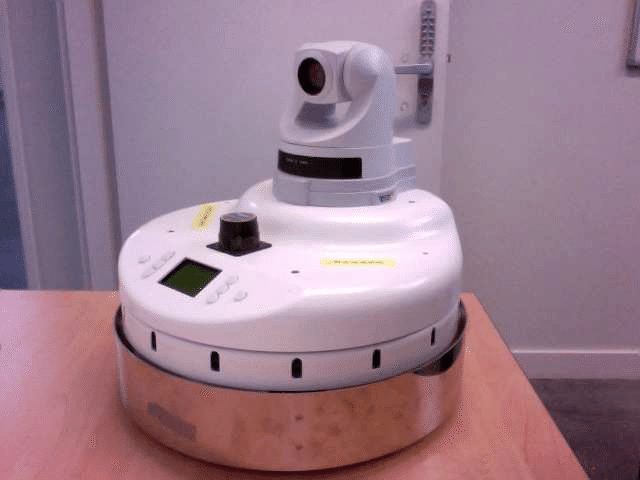
\includegraphics[scale=0.5]{pekee.png}
	\captionof{figure}{\textit{Robot pekee II\\}}
	\label{fig1} 
	\end{center}   
	